% multipath execution on a large-scale distributed microarchitecture
%
\documentclass[10pt,twocolumn,dvips]{article}
\usepackage[english]{babel}
\usepackage{epsfig}
%\usepackage{fancyheadings}
%\usepackage[T1]{fontenc}
%\usepackage[latin1]{inputenc}
%\usepackage{twocolumn}
%\usepackage{verbatim,moreverb,doublespace}
%\usepackage{rotate,lscape,dcolumn,array,rotating,latexsym}
%
%\input{epsf}
%\textwidth 175mm
\textwidth 6.6in 
\textheight 239mm
%\leftmargin -2.0in
%\textheight 225mm
%\topmargin -15mm
\topmargin -4.5mm
%\oddsidemargin 0mm
%\evensidemargin 0mm
%
\pagestyle{empty}
%
\begin{document}
\parskip 1mm
%
%
\title{Mutlipath Execution on a Large-Scale Distributed 
Microarchitecture}
%
\author{
D.R. Kaeli, A. Khalafi, D. Morano\\
Northeastern University\\
{kaeli, akhalafi, dmorano}@ece.neu.edu\\
\and
A.K. Uht \\
University of Rhode Island\\ uht@ele.uri.edu
}
% For a paper whose authors are all at the same institution,
% omit the following lines up until the closing ``}''.
% Additional authors and addresses can be added with ``\and'',
% just like the second author.
%
\date{ }
\maketitle
\date{ }
\thispagestyle{empty}
%
\begin{abstract}
\footnotesize{
This paper explores the implementation of multipath execution on a
large distributed microarchitecture.  With the advent of the
possibility of large microarchitures, means to mitigate, or help to
mitigate, the deleterious effects of branch mispredictions need to be
more aggressively explored.  We suggest that multipath execution is one
way to approach the continuing problem of branch misprediction
penalties.  Further, with a microarchitecture that now allows for very
large numbers of instrcutions to be simultaneously in the process of
being executed, multipath execution provides a more efficient use of
hardware execution resources than continuing to speculatively execute
hundreds or more instructions down a single path.

We briefly present the outline of a large scale distributed microarchitecture
and discuss how we overlay multipath execution on it.
We provide simulation results for several microarchitectural configurations
that demonstrate the positive effects of multipath execution in
hiding and mitigating the inevitable branch mispredictions.
}
\end{abstract}
%
\vspace{-0.2in}
\section{Introduction}
\vspace{-0.1in}
A number of studies into the limits of instruction level parallelism (ILP) have
been promising in that they have shown that there is parallelism within
typical programs~\cite{Gon97,Lam92,Uht95}.  
Unfortunately, most of this fine-grained
parallelism spans several basic blocks and the relatively small
instruction fetch windows of existing processor designs cannot span
the program instruction space necessary to begin to exploit this
parallelism.  A large number of instructions need to be fetched
each cycle and executed concurrently in order to expose this ILP.
A fundamental challenge 
is how to find this parallelism and then allow execution to occur
out of order  
while still maintaining the architectural program order that
is required for proper program execution.
We need to find this ILP at runtime; we need to 
enable the hardware to find, schedule,
and otherwise manage possible control and data independent instructions.

A large, distributed, microarchitecture, capable of executing tens or
hundreds of instructions concurrently
is needed in order to exploit the fine-grained parallelism present 
in integer programs (e.g., SPECint2000).
A barrier encountered when realizing a large-scale microarchitectures is the
competition for centralized machine resources.
These resources often include the 
physical register file (including both architectural as well as renaming 
registers), register renaming logic,
and the reorder buffer.  Other resources that are often centralized
in conventional microarchitectures are the execution units, though they
do not present the same challenges for maintaining correct program order
as those resources that are associated with the architected registers
and the dependencies (control, register, and memory) that arise
from the instructions themselves.  The use of centralized resources
greatly hinders the scalability of any microarchitecture implementation. 

We present a microarchitecture that is able to scale to large sizes
through the
elimination of most conventional centralized microarchitectural components.
We are proposing to use time tags to maintain 
and enforce correct program order for all flow dependencies whether
they be registers, memory values, or instruction control-flow predicates.
A description of the general microarchitecture
assumed in this paper is presented in~\cite{Uht01}.  In this paper
we focus our attention on the design of time tags.

Section 2 will discuss a basic distributed microarchitecture that
achieves the above goals and how time tags are defined and used
to coordinate its execution flow.  
Section 3 discusses some of the differences between our envisioned
microarchitecture and existing schemes.
Section 4 presents a small set of simulation results that demonstrate
the power of using time tags. 
Section 5 
summarizes the current contributions.
%\vspace{-0.3in}
\section{Distributed Microarchitecture Using Time Tags}
\vspace{-0.1in}
In order to achieve high IPC in single-threaded, branch-dominated 
program codes, many instructions need to be examined and executed
in parallel.  We desire that the span of instructions that might be
executed in parallel be on the order of at least tens and possibly hundreds
or thousands.  Unfortunately, having a large numbers of instructions
in flight simultaneously places an enormous burden on access to 
the physical register file (or files, if they are partitioned in some way),
the architected register mapping function, and the reorder buffer 
needed for
management of the final committed program order.
\vspace{-0.2in}
\subsection{Active Stations and Execution Window}
\vspace{-0.1in}
To address contention problems encountered with centralized
machine resources, we have extended the idea of Tomasulo's reservation
station \cite{Tom67} to provide the basic building block for a distributed
microarchitecture.  Tomasulo's reservation station provides for the
simultaneous execution of different instructions over several
functional units.  This part of his scheme (already widely used) is
retained but extended to forward execution results to other spatially
separated and distributed reservation stations and execution units
rather than looping the results back to a common instruction issue unit
and update logic for the architected register file.  We also extend the idea
of the reservation station to allow for multiple executions (re-executions)
of the same instruction in the station.  We will keep an 
instruction in the station until it is retired (either committed or 
squashed).  
We call our adaptation of the reservation station an 
{\em Active Station}(AS).  

Rather than lay our Active Stations out in silicon simply next to
the functional units that will execute the instructions issued to them,
we will lay them out in a two dimensional grid whereby sequentially
issued instructions are assigned to sequential ASes down a column of
the two dimensional grid of ASes.  The two dimensional
grid of ASes, along with their interspersed execution units,
is called the {\em Execution Window}.
We issue instructions to the ASes simultaneously, a column at
a time.  We attempt to issue every cycle.
To manage control, register data, and memory
data dependencies, we make extensive use of time tags.

Fortunately, our present model for program execution provides
a very key advantage to exploiting a large and distributed microarchitecture.
Since inorder issued instructions 
only need to forward (versus backward) results into the
program-ordered future, there is no real need to provide connectivity
to previously executed instructions 
(previous in program order).  This is the basic
idea of laying out the active stations in columns.  Result operands
from one instruction will flow forward to the next program instructions
that are in the ordered future of the program (whether those
instructions are speculative or not).  
Groups of active stations
that share execution resources are termed \textit{Sharing Groups}.
\vspace{-0.2in}
\subsection{Time Tags and Renaming}
\vspace{-0.1in}
A time tag indicates
the position of an instruction in the original 
sequential program order (i.e., in the order that instructions are issued
to active stations).  
Active stations are labeled with time tags starting
from zero and incrementing up to one minus the total number of
active stations in the microarchitecture.  
A time tag is a small
integer that uniquely identifies a particular active station.
Time tags can be thought of as having two
parts.  Since the active stations are laid out
in columns and rows, time tags can be viewed as having a column
component and a row component.  The column component 
occupies the high order bits of
the time tag integer and the row component occupies the remaining space.

For illustrative purposes, we usually assign time tags, starting with the
value zero,
to active stations starting at the upper left corner of the two
dimensional grid of active stations and proceed to assign incremented
time tags first down the left-most column and continuing down the
next column to its right until all active stations are numbered.
The reader is again referred to~\cite{Uht01} for possible
active station configuration options. 

Similarly to the conventional reservation station, operand results
are broadcast forward for use by waiting instructions.
With active stations, all operands that are forwarded after the execution
of an instruction are also tagged with the time tag value of the
active station that generated the updated operand.
This tag will be used by subsequent active stations to determine if
the operand should be {\em snarfed}~\footnote{snarfing entails snooping
address/data buses, and when the desire address value is detected, 
the associated data value is read} 
as an input operand that will trigger
the execution of its loaded instruction.

Essentially all values within the execution
window are tagged with time tags.
Since our microarchitecture can also allow for the concurrent
execution of multiple speculative paths of the current program,
we also introduce a path identifier (path ID).
A path ID 
identifies the current path that an active station is executing an instruction
for.  
Path IDs are numbered from zero
to one minus the total number of possible paths.
Path IDs are assigned to all operands in the execution window
along with time tags.

The microarchitecture that we have devised requires the
forwarding of three types of operands.  These are register
operands, memory operands, and instruction predicate operands.
These operands are tagged with time tags and path IDs that were associated
with the active stations that produced them.
The information 
broadcast from an AS to subsequent
ASes in future program ordered time is referred
to as a {\em transaction}, and consists of :
\vspace{-0.05in}
\begin{itemize}
\vspace{-0.1in}
\item{a path ID}
\vspace{-0.1in}
\item{the time tag of the originating active station}
\vspace{-0.1in}
\item{the identifier of the architected operand}
\vspace{-0.1in}
\item{the actual data value for this operand}
\vspace{-0.1in}
\end{itemize}   

Figure \ref{fig:source} shows the registers inside an active
station for one of its input operands.  The 
{\em time-tag},
{\em address}, and
{\em value} registers are reloaded with new values on each snarf,
while the
{\em path} and
{\em AS time-tag} are only loaded when the active station is
issued an instruction.
The operand shown is typical for source registers, a source memory
operand, or an instruction execution predicate register.
\begin{figure}
\centering
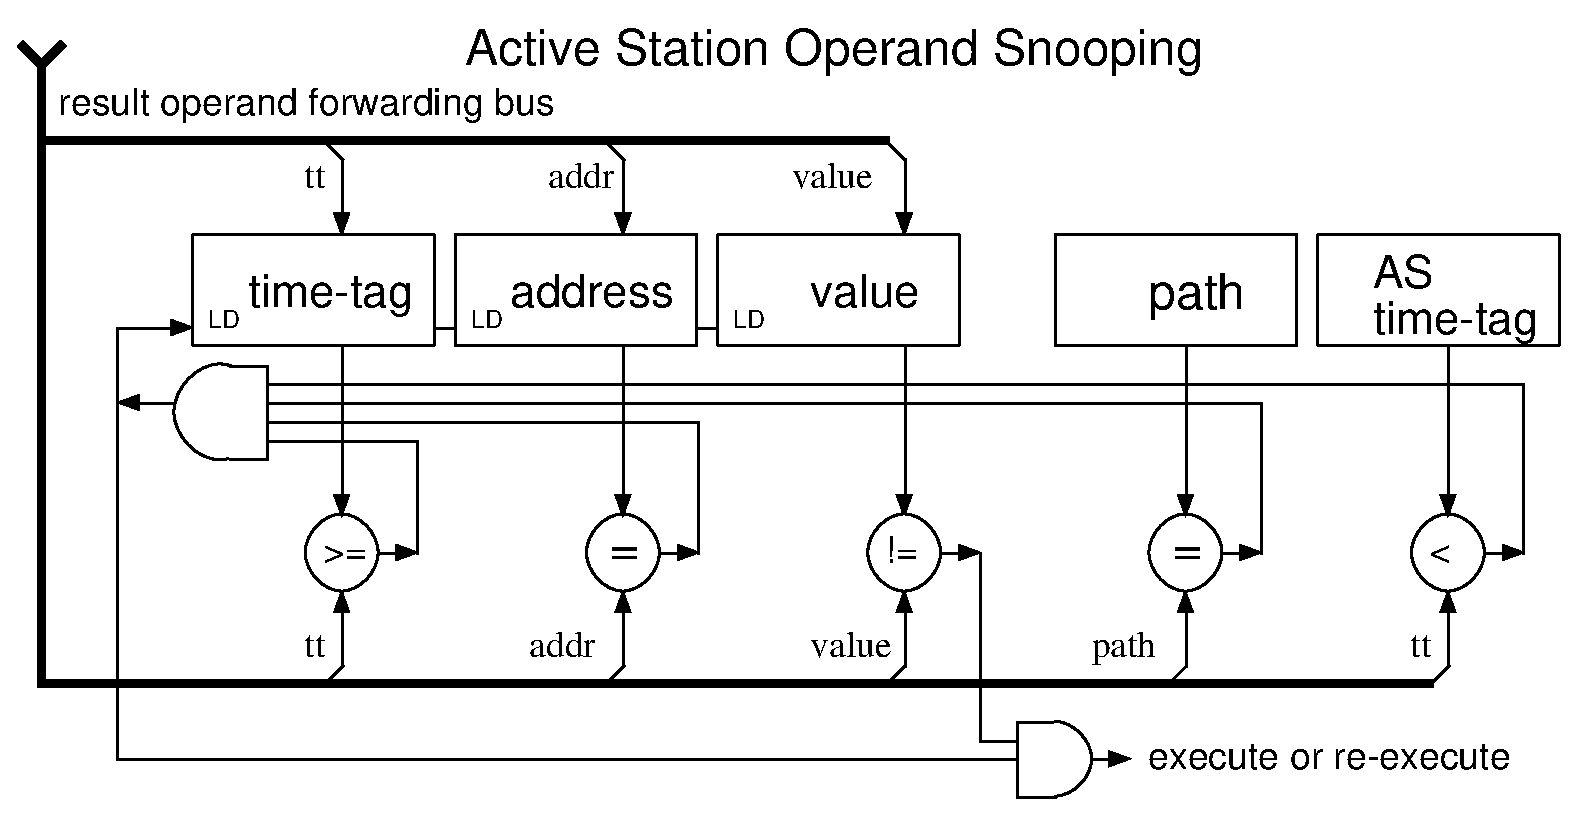
\epsfig{file=source.eps,width=3.0in}
\caption{{\em Active Station Source Operand.} The registers and snooping
operation of one of several possible source operands is shown.
Just one operand forwarding bus is shown being snooped but
typically several operand forwarding buses are snooped simultaneously.}
\label{fig:source}
\end{figure}
In the case of a register operand being forwarded, the name of the
operand is the address of the architected register.  For example
if the architected register in question is {\tt r6} then the
name of that operand would be the value 6.  If the operand
being forwarded is a memory operand, then the name of the operand
is simply its address (either a 32-bit address or a 64-bit address
depending on the machine ISA).  If the operand is a predicate,
then the name might be an internally derived value depending on
the predication implementation. 

This scheme effectively eliminates the need for rename registers
or other speculative registers as part of the reorder buffer.
The whole of the microarchitecture thus provides for the full renaming
of all operands, thus avoiding all false dependencies.
There is no need to limit instruction issue or to limit speculative
instruction execution due to a limit on the number of non-architected
registers for holding those temporary results.

True flow dependencies are enforced through continuous  
snooping by each active station.  Each active station
will snoop all operands that are broadcast to it.  If the
path ID and the architected name of the operand match any of
its current input operands, the active station then checks
if the time tag value is less than its own assigned time tag,
and greater than or equal to the time tag value of the last
operand that it snarfed, if any.  If the snooped data value is
different than the input operand data value that the active
station already has, a re-execution of the instruction is initiated.
This simple rule will enforce
all proper flow dependencies while allowing for massive
concurrency to occur.
\vspace{-0.2in}
\subsection{Result Forwarding Buses}
\vspace{-0.1in}
There are several choices for a suitable interconnection fabric between
the active stations.  Our fabric uses segmented buses with buffers
between stages; this preserves
scalability and provides reasonable performance (we exploit the fact
that register lifetimes only span 1 or 2 basic blocks).
This paper will not address the
many options that are available.  The purpose of the
interconnection fabric is to primarily forward instruction result
operands, tagged with their time tags, 
to those active stations in the program ordered future (those
active stations with higher valued time tags).  This means that one
basic requirement of the interconnection fabric is that it must be able
to transport operand results from any active station in a column to
those active stations lower in the column and then to the remaining
active stations to the right of the current column starting again at
the top of the next column to the right.  So regardless of the number
and types of connections for interconnecting buses, the buses must
allow for the flow of operands from top left-most active station in the
grid, down the left-most columns of ASes, up to the top of the next and
repeating for all columns.

It must be noted at this point that operand result forwarding
bus connectivity is also needed (in a seemless way) from the bottom
right-most active station to the top left-most active station.
This is needed because assignment of time tags (as discussed so far)
is not going to remain static during the actual operation of the machine.
As columns of ASes retire and new columns are issued new instructions,
all of the time tags in the execution window are decremented by
an amount equal to the numbers of ASes in a column.  This corresponds
to decrementing the column part of each time tag in the whole of the
execution window by one.  Newly issued instructions will take on
time tag values corresponding to the right-most 
column of ASes.  The oldest column becomes the 
newest column; columns are connected by a toridal network in the
execution window.
\vspace{-0.2in}
\section{Related Approaches}
\vspace{-0.1in}
The Warp Engine~\cite{Cleary95} used time tags; however their implementation
is cumbersome, utilizing floating point numbers and machine wide parameter
updating.  The Metaflow Architecture discusses the 
idea of {\em delayed scheduling}
to obtain moderate gains in ILP~\cite{Pop}.

By developing a microarchitecture based around active stations
and the use of time tags to coordinate and enforce correct program
order, we eliminate the need for the severe contention present 
on either register scoreboards \cite{Thornton64} 
or the architected register files associated
with the use of reservation stations~\cite{Anderson67}.  

In those microarchitectures
that perform speculative execution, there is also
the need to access the reorder buffer, which becomes quite problematic
as the number of instructions being speculatively executed concurrently
grows~\cite{Palacharla}.  Whether speculative instruction operand
results are stored in data registers within the reorder buffer or if the
results are stored in extra physical registers that hold both architected
and temporary values, the contention for the centralized resource is
the same.  In our microarchitecture, the set of active
stations form a giant reorder buffer.  The registers that
make up a reorder buffer in a conventional microarchitecture are
not eliminated entirely in the sense that we store the same speculative
information in a distributed way in each active station.  Similarly,
although the need for centralized rename registers is eliminated,
we are effectively storing the rename registers along with the
decoded instructions inside each active station.  
\vspace{-0.2in}
\section{IPC Results}
\vspace{-0.1in}
We report execution-driven simulation results for  
SpecInt-2000 and SpecInt-95 programs run on a 
simulated time-tagged microarchitecture 
that executes SGI-MIPs binaries. 
The data in Table 1 contains IPC results for a range of machine sizes
and configurations. 
The general features of
the machine simulated are 100\% hit rates for L1 instruction cache,
a 1 cycle hit delay and 10 cycle miss penalty for the L1 data cache,
100\% hit in the L2 data cache, an operand forwarding delay of 1 clock
per stage
and a general bus stage delay of 1 clock.  The data cache is 32KB 2-way
set associative that is also 4-way interleaved.
Each of the machine configurations in Table \ref{tab:ipc} consists of three
numbers that give the rows of sharing groups, the number
of active station rows per sharing group, and the total number of 
columns respectively.  The number of sharing group rows times the
number of active stations per sharing group is the total number of
active stations rows in a configuration.  
\begin{table}
\footnotesize{
\begin{center}
\begin{tabular}{|c|c|c|c|c|c|c|}
\hline 
config&
4-4-4&
8-4-4&
8-4-8&
8-8-8&
16-8-4&
8-4-16\\
\hline
\hline 
bzip2&
2.7&
3.9&
4.3&
5.1&
4.5&
4.9\\
\hline 
parser&
2.6&
3.9&
4.8&
5.7&
4.4&
5.3\\
\hline 
gzip&
2.8&
4.0&
4.6&
5.8&
5.2&
5.6\\
\hline 
gap&
3.3&
4.9&
5.9&
6.5&
5.8&
6.0\\
\hline 
go&
2.9&
4.2&
5.4&
6.3&
4.8&
5.6\\
\hline 
hmean&
2.8&
4.2&
4.9&
5.8&
4.9&
5.4\\
\hline
\end{tabular}
\end{center}
}
\caption{Benchmark IPC results for various machine sizes.}\label{tab:ipc}
\end{table}

As can be seen from the data, the configuration of 8-8-8 provides
the best overall IPC for the configurations simulated.  This consists
of 64 active stations in each column with 8 columns.
Configuration 16-8-4 does not perform as well because it does not
have as many columns (only 4 as compared with 8 in the other configuration)
to hide the latencies of instruction execution.  Eight columns 
hides more instruction execution latency than four.  The 8-4-16
configuration performs poorly as compared with 8-8-8 because the height
of a column (the primary IPC multiplier) is only 32 and its extra
columns are not needed to hide more instruction execution latency.
\vspace{-0.2in}
\section{Summary}
\vspace{-0.1in}
We have presented a new microarchitecture, extended from Tomasulo's
reservations stations, that uses time tags to coordinate and enforce
program order on large-scale out of order execution.
The use of time tags allows for the scalability of our microarchitecture
to sizes that can allow for hundreds of instructions (or more) to execute
concurrently.
Our results indicate that this general approach appears to be quite
promising as compared with the existing more conventional microarchitectural
approaches.  Some work on much larger machine configurations has already
suggested that achieving IPC numbers in the 10s on general integer
sequentially-oriented program codes is possible.
\vspace{-0.1in}
\bibliographystyle{latex8}
\bibliography{timetags}
\end{document}
